\documentclass[aspectratio=169,12pt]{beamer}
\usepackage[utf8]{inputenc}
\usepackage{amsmath, amssymb}
\usepackage{booktabs}
\usepackage{hyperref}
\usepackage{tikz}
\usepackage{graphicx}
\usepackage{listings}
\usepackage{tcolorbox}
\usepackage{minted}
\usetikzlibrary{arrows.meta, positioning, shapes.geometric, calc, fit, shapes.callouts, tikzmark}
\usetheme{Madrid}

% Define colors
\definecolor{codegreen}{RGB}{40,180,99}
\definecolor{codepurple}{RGB}{155,89,182}
\definecolor{codeorange}{RGB}{230,126,34}
\definecolor{lightgray}{RGB}{245,245,245}
\definecolor{calloutbg}{RGB}{255,255,200}
\definecolor{keybg}{RGB}{255,220,180}

\lstset{
    basicstyle=\ttfamily\small,
    breaklines=true,
    backgroundcolor=\color{lightgray}
}

\title{Agentic Programming with LLMs}
\author{Computer Architecture 2360267}
\date{2025, Administrative \#0}

\begin{document}

\frame{\titlepage}

%======================================================================
\begin{frame}{Outline}
\tableofcontents

\vspace{0.3cm}
{\small \textcolor{gray}{Appendix: Claude Code Setup (alternative tool)}}
\end{frame}

%======================================================================
\section{Introduction}
%======================================================================

\begin{frame}{Pilot Program: LLM-Assisted Assignments}

\textbf{New this semester:} Part of the home assignments will be ``wet'' (programming) assignments.

\vspace{0.5cm}

As part of a \textbf{pilot program}, students are expected to use Large Language Models (LLMs) for these assignments:

\begin{itemize}
    \item Each pair receives \textbf{\$10 credit} via \href{https://openrouter.ai}{OpenRouter.ai}
    \item \textbf{Tool options:} \href{https://opencode.ai}{OpenCode.ai} (recommended) or Claude Code (see \hyperref[sec:appendix]{Appendix})
    \item \textbf{Model choices:} GLM-4.7 or Kimi K2 Thinking
    \item Goal: Learn \textbf{agentic AI programming} workflows
\end{itemize}

\vspace{0.3cm}

\textbf{Why?} AI-assisted development is becoming an essential skill for engineers. This pilot helps you gain hands-on experience.

\vspace{0.3cm}

{\small \textcolor{codeorange}{\textbf{Note:}} Both tools connect to OpenRouter and use your API key. Choose whichever interface you prefer!}

\end{frame}

%======================================================================
\begin{frame}{What is Agentic AI Programming?}

\textbf{Agentic AI} = AI that can autonomously perform multi-step tasks

\vspace{0.3cm}

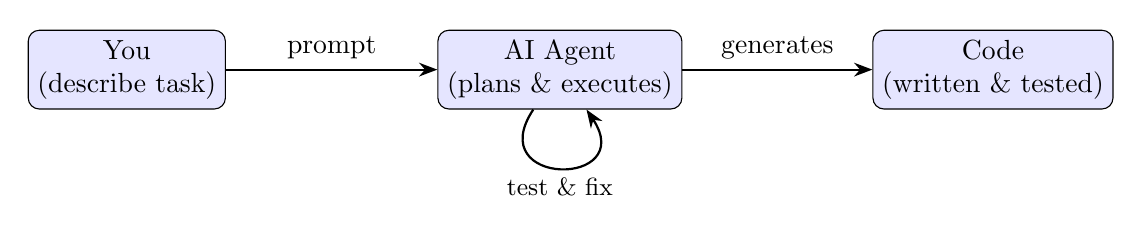
\begin{tikzpicture}[
    box/.style={draw, rounded corners, fill=blue!10, minimum width=2.5cm, minimum height=1cm, align=center},
    arrow/.style={->, thick, >=Stealth}
]
    \node[box] (user) at (0,0) {You\\(describe task)};
    \node[box] (agent) at (5.5,0) {AI Agent\\(plans \& executes)};
    \node[box] (code) at (11,0) {Code\\(written \& tested)};

    \draw[arrow] (user) -- (agent) node[midway, above] {prompt};
    \draw[arrow] (agent) -- (code) node[midway, above] {generates};

    % Self-loop: agent tests, sees errors, fixes, repeats
    \draw[arrow] (agent) .. controls (4.5,-1.5) and (6.5,-1.5) .. node[below,font=\small] {test \& fix} (agent);
\end{tikzpicture}

\vspace{0.5cm}

Unlike simple chatbots, agentic AI can:
\begin{itemize}
    \item Read and navigate your codebase
    \item Write, edit, and delete files
    \item Run commands and tests
    \item Fix errors and iterate until the task is complete
\end{itemize}

\end{frame}

%======================================================================
\section{Setup}
%======================================================================

\begin{frame}{Getting Your API Key}

\textbf{Step 1: Submit HW0 via \href{https://webcourse.cs.technion.ac.il/02360267}{Webcourse}}
\begin{itemize}
    \item Provide your details (name, ID, email)
    \item Provide your partner's details (if working in pairs)
\end{itemize}

\vspace{0.5cm}

\textbf{Step 2: Receive Your API Key}
\begin{itemize}
    \item After HW0 submission, you will receive your personal API key via \href{https://webcourse.cs.technion.ac.il/02360267}{Webcourse}
    \item Key format: \texttt{sk-or-v1-...}
    \item \textbf{Keep this key private!} Do not share it.
\end{itemize}

\vspace{0.5cm}

\textbf{Budget:} \$10 per pair --- should suffice for all assignments, but monitor usage!

\end{frame}

%======================================================================
\subsection{OpenCode.ai Setup}
%======================================================================

\begin{frame}[fragile]{Installing OpenCode.ai}

\textbf{Recommended Installation:}
\begin{minted}[fontsize=\scriptsize,bgcolor=lightgray]{bash}
curl -fsSL https://opencode.ai/install | bash
\end{minted}

\vspace{0.3cm}

\textbf{Alternative --- Homebrew (macOS/Linux):}
\begin{minted}[fontsize=\scriptsize,bgcolor=lightgray]{bash}
brew install anomalyco/tap/opencode
\end{minted}

\vspace{0.3cm}

\textbf{Alternative --- npm (requires Node.js 18+):}
\begin{minted}[fontsize=\scriptsize,bgcolor=lightgray]{bash}
npm install -g opencode
\end{minted}

\vspace{0.3cm}

{\footnotesize
\textbf{Documentation:} \url{https://opencode.ai/docs}\\
Additional installation options (Docker, pnpm, etc.) available in the docs.
}

\end{frame}

%======================================================================
\begin{frame}[fragile]{Configuring OpenCode.ai for OpenRouter}

\textbf{Step 1:} Open a terminal and run:
\begin{minted}[fontsize=\footnotesize,bgcolor=lightgray]{bash}
opencode
\end{minted}

\vspace{0.3cm}

\textbf{Step 2:} Inside OpenCode, type \colorbox{lightgray}{\texttt{/connect}} and press Enter

\vspace{0.3cm}

\textbf{Step 3:} Search for ``OpenRouter'' in the provider list

\vspace{0.3cm}

\textbf{Step 4:} Paste your API key when prompted:
\begin{itemize}
    \item Format: \texttt{sk-or-v1-...}
    \item This is the key you received from \href{https://webcourse.cs.technion.ac.il/02360267}{Webcourse}
\end{itemize}

\vspace{0.3cm}

{\small \textcolor{codeorange}{\textbf{Note:}} Keep your API key private! Do not share it with others.}

\end{frame}

%======================================================================
\begin{frame}[fragile]{Choosing Your Model}

After connecting to OpenRouter, select your model:

\vspace{0.3cm}

\textbf{Type} \colorbox{lightgray}{\texttt{/models}} \textbf{and choose one of these:}

\vspace{0.3cm}

\begin{itemize}
    \item \href{https://z.ai/blog/glm-4.7}{\textbf{GLM-4.7}}
    \begin{itemize}
        \item Cost: \$0.40/M input, \$1.50/M output tokens
        \item Context: 203K tokens
        \item Fast, good for iterative development
    \end{itemize}

    \vspace{0.2cm}

    \item \href{https://www.kimi.com/en}{\textbf{Kimi K2 Thinking}}
    \begin{itemize}
        \item Cost: \$0.57/M input, \$2.42/M output tokens
        \item Context: 256K tokens
        \item Shows step-by-step reasoning
    \end{itemize}
\end{itemize}

\vspace{0.3cm}

{\small You can switch models anytime using \colorbox{lightgray}{\texttt{/models}}}

\end{frame}

%======================================================================
\begin{frame}[fragile]{Verifying Your OpenCode.ai Setup}

\textbf{Step 1:} Check the status bar at the bottom

\vspace{0.2cm}

The status bar should display your current model:
\begin{center}
\colorbox{lightgray}{\texttt{GLM-4.7 (OpenRouter)}} or \colorbox{lightgray}{\texttt{Kimi K2 Thinking (OpenRouter)}}
\end{center}

\vspace{0.3cm}

\textbf{Step 2:} Test with a simple prompt:

\vspace{0.2cm}

\begin{minted}[fontsize=\footnotesize,bgcolor=lightgray]{text}
You: "Hello! Can you see my current directory?"
\end{minted}

\vspace{0.3cm}

If OpenCode responds correctly, you're all set!

\vspace{0.3cm}

{\small \textcolor{codegreen}{\textbf{Tip:}} Use \colorbox{lightgray}{\texttt{/help}} to see all available commands.}

\end{frame}

%======================================================================
% Hidden slide: Manual budget checking via curl (requires shell variables)
\iffalse
\begin{frame}[fragile]{Checking Your Budget (Manual)}\label{frame:budget}

\vspace{-0.2cm}
If you have \texttt{ANTHROPIC\_AUTH\_TOKEN} exported in your shell, run:
\begin{minted}[fontsize=\footnotesize,bgcolor=lightgray]{bash}
curl https://openrouter.ai/api/v1/auth/key \
     -H "Authorization: bearer $ANTHROPIC_AUTH_TOKEN" | jq
\end{minted}

\vspace{0.1cm}

Example output:
\begin{minted}[fontsize=\scriptsize,bgcolor=lightgray]{json}
{
  "data": {
    "label": "sk-or-v1-852...8dd",
    "limit": 10.0,
    "limit_remaining": 9.59,
    "usage": 0.408003788,
    ...
  }
}
\end{minted}

\vspace{0.1cm}

\textbf{Key fields:}
\begin{itemize}
    \item \texttt{usage}: Total amount spent so far (in USD)
    \item \texttt{limit\_remaining}: How much budget you have left
\end{itemize}

\end{frame}
\fi

%======================================================================
\begin{frame}[fragile]{Checking Your Budget}

\textbf{Both tools use your OpenRouter budget.} Monitor it to avoid running out!

\vspace{0.5cm}

\textbf{Check your remaining budget at:}
\begin{center}
\large\url{https://nadav.amit.zone/tools/openrouter-budget.html}
\end{center}

\vspace{0.3cm}

{\small Enter your API key (\texttt{sk-or-v1-...}) to see your remaining balance.}

\vspace{0.5cm}

{\small \textcolor{codeorange}{\textbf{Note:}} No extra budget will be provided. Monitor your usage!}

\end{frame}

%======================================================================
\begin{frame}[fragile]{IDE Integration}

\textbf{Running OpenCode.ai in your IDE:}
\begin{itemize}
    \item Run \colorbox{lightgray}{\texttt{opencode}} directly in your IDE's terminal
    \item Works with VSCode, Cursor, or any editor with a terminal
    \item Open terminal:
    \begin{itemize}
        \item \textbf{VSCode/Windows:} \colorbox{keybg}{\texttt{Ctrl+Shift+`}}
        \item \textbf{macOS:} \colorbox{keybg}{\texttt{Cmd+`}}
    \end{itemize}
\end{itemize}

\vspace{0.3cm}

\textbf{Benefits:}
\begin{itemize}
    \item AI sees your open files and workspace context (type \colorbox{lightgray}{\texttt{/ide}} to check)
    \item Easy to review changes in your editor
    \item Natural integration with your existing workflow
\end{itemize}

\vspace{0.3cm}

{\small \textcolor{codeorange}{\textbf{WSL users:}} Set default terminal to WSL: \colorbox{keybg}{\texttt{Ctrl+Shift+P}} $\rightarrow$ ``Terminal: Select Default Profile'' $\rightarrow$ choose your WSL distribution.}

\vspace{0.2cm}

{\small For Claude Code IDE integration, see the \hyperref[sec:appendix]{Appendix}.}

\end{frame}

%======================================================================
\section{Best Practices}
%======================================================================

\begin{frame}{Tips for Effective Prompting}

\textbf{1. Be Specific About Context}
\begin{itemize}
    \item ``Write a Verilog module for a 5-stage pipeline latch''
    \item Not: ``Help me with my assignment''
\end{itemize}

\vspace{0.3cm}

\textbf{2. Break Down Complex Tasks}
\begin{itemize}
    \item Start with the interface/specification
    \item Then implement components incrementally
    \item Test each part before moving on
\end{itemize}

\vspace{0.3cm}

\textbf{3. Provide Examples}
\begin{itemize}
    \item Show input/output examples when possible
    \item Reference existing code patterns in your project
\end{itemize}

\end{frame}

%======================================================================
\begin{frame}{Test-Driven Development with AI}

\textbf{4. Write Tests Early!}
\begin{itemize}
    \item Ask the AI to write tests \textbf{before} or \textbf{alongside} implementation
    \item ``First write a testbench for this module, then implement it''
    \item Verify tests pass at each stage
\end{itemize}

\vspace{0.3cm}

\textbf{5. Run Tests Iteratively}
\begin{itemize}
    \item For complex tasks: run tests after \textbf{every significant change}
    \item Let the AI see test failures and fix them immediately
    \item Don't wait until the end to discover problems!
\end{itemize}

\vspace{0.3cm}

\textbf{6. Use \colorbox{lightgray}{\texttt{AGENTS.md}} for Project Context}
\begin{itemize}
    \item Create an \colorbox{lightgray}{\texttt{AGENTS.md}} file in your project root
    \item Or use \colorbox{lightgray}{\texttt{/init}} in OpenCode.ai to generate it automatically
    \item Document: build commands, test commands, project structure
    \item The AI reads this file automatically for context
\end{itemize}

\end{frame}

%======================================================================
\begin{frame}[fragile]{Project Context Files}

\textbf{OpenCode.ai uses} \colorbox{lightgray}{\texttt{AGENTS.md}} \textbf{in your project root:}

\vspace{0.2cm}

\begin{itemize}
    \item Generate automatically: run OpenCode.ai, type \colorbox{lightgray}{\texttt{/init}}
    \item Or create manually with build commands, project structure, etc.
    \item OpenCode.ai reads this file automatically for context
\end{itemize}

\vspace{0.3cm}

{\small \textbf{Claude Code} uses \colorbox{lightgray}{\texttt{CLAUDE.md}} instead (see \hyperref[sec:appendix]{Appendix}).}

\vspace{0.3cm}

\textbf{Example content:}

\begin{minted}[fontsize=\scriptsize,bgcolor=lightgray]{markdown}
# Build commands
- make: Build the project
- make test: Run all tests
- make debug: Build with debug symbols (-g)
- gdb ./program: Debug with GDB

# Code style
- Use meaningful variable names
- Comment non-obvious bit manipulations

# Project structure
- src/: C source files
- include/: Header files
- tests/: Test cases
\end{minted}

\vspace{0.2cm}

\textbf{Benefits:} The AI reads this automatically $\rightarrow$ better context, fewer mistakes.

\vspace{0.1cm}

{\footnotesize Resources: \url{https://www.anthropic.com/engineering/claude-code-best-practices} (for Claude Code), or use OpenCode's \colorbox{lightgray}{\texttt{/init}} to generate \texttt{AGENTS.md}}

\end{frame}

%======================================================================
\begin{frame}{Planning Mode}

For complex tasks, ask the AI to \textbf{plan before implementing}:

\vspace{0.3cm}

\textbf{Claude Code:}
\begin{itemize}
    \item Press \colorbox{keybg}{\textbf{Shift+Tab}} to toggle plan mode
    \item Or ask: ``Plan how to implement X before writing code''
\end{itemize}

\textbf{OpenCode.ai / General approach:}
\begin{itemize}
    \item Ask: ``Plan how to implement X. Don't write code yet, explain the approach''
    \item Review the plan, suggest changes, then proceed
\end{itemize}

\vspace{0.3cm}

\textbf{Benefits:}
\begin{itemize}
    \item Catch architectural issues early
    \item Ensure the AI understands the requirements
    \item Save tokens/budget by avoiding wrong directions
\end{itemize}

\end{frame}

%======================================================================
\begin{frame}{Version Control: Rewind and Git}

\textbf{Claude Code:} Built-in \colorbox{lightgray}{\texttt{/rewind}} (CLI only)
\begin{itemize}
    \item Useful if the AI takes a wrong direction
    \item Not available in VSCode extension or OpenCode.ai
\end{itemize}

\vspace{0.3cm}

\textbf{Git: Universal Safety Net (Works with Both Tools)}
\begin{itemize}
    \item \textbf{Commit frequently} before asking AI to make big changes
    \item If something goes wrong: \colorbox{lightgray}{\texttt{git checkout .}} or \colorbox{lightgray}{\texttt{git reset}}
    \item Create branches for experimental features
\end{itemize}

\vspace{0.3cm}

\textbf{Recommended workflow:}
\begin{enumerate}
    \item \colorbox{lightgray}{\texttt{git commit}} your working state
    \item Ask AI to implement feature
    \item If happy: commit the changes
    \item If not: \colorbox{lightgray}{\texttt{git checkout .}} to revert
\end{enumerate}

\end{frame}

%======================================================================
\section{Safety and Permissions}
%======================================================================

\begin{frame}[fragile]{Sandboxing}

\textbf{Sandboxing} = OS-level filesystem \& network isolation for safer operation.

\vspace{0.3cm}

\textbf{What it does:}
\begin{itemize}
    \item \textbf{Filesystem:} Write access only to working directory; read access elsewhere
    \item \textbf{Network:} Only approved domains can be accessed
    \item Prevents accidental damage to your system
\end{itemize}

\vspace{0.3cm}

\textbf{OpenCode.ai with Docker (recommended for sandboxing):}
\begin{minted}[fontsize=\scriptsize,bgcolor=lightgray]{bash}
docker run -it --rm -v $(pwd):/workspace ghcr.io/anomalyco/opencode
\end{minted}
{\small Runs OpenCode.ai in an isolated container with your current directory mounted.}

\vspace{0.3cm}

{\small For Claude Code sandboxing options, see the \hyperref[sec:appendix]{Appendix}.}

\end{frame}

%======================================================================
\section{Context Management}
%======================================================================

\begin{frame}{Understanding Context Windows}

\vspace{-0.2cm}
\textbf{Context window} = the AI's ``working memory'' for your conversation.

\begin{itemize}
    \item Everything you send (prompts, code, errors) fills the context
    \item The AI also uses context for its ``thinking'' and responses
    \item \textbf{Finite resource:} When full, quality degrades $\rightarrow$ start fresh!
    \item Some models give worse answers as context fills (``context anxiety'')\footnote{See: \url{https://inkeep.com/blog/context-anxiety}}
\end{itemize}

\vspace{0.1cm}

\textbf{Context compaction (Claude Code):} Claude Code automatically summarizes older parts of the conversation when context fills up. You may see ``Compacting...'' or ``This session is being continued...''
\begin{itemize}
    \item Details from early in the session may become less precise
    \item Important decisions might need to be restated
    \item OpenCode.ai handles context differently --- monitor manually
\end{itemize}

\vspace{-0.1cm}

\textbf{Cost implications:} Larger context = more tokens = higher cost.\footnote{Even with KV-cache optimizations, you pay for the full context on each turn.}

\end{frame}

%======================================================================
\begin{frame}{When to Start a Fresh Session}

\textbf{Signs you should start a new session:}
\begin{itemize}
    \item Switching to a completely different task
    \item AI starts making mistakes about earlier code
    \item You've been going for 30+ turns on complex work
    \item Claude Code shows context usage warnings
\end{itemize}

\vspace{0.3cm}

\textbf{How to start fresh:}
\begin{itemize}
    \item \colorbox{lightgray}{\texttt{/clear}} --- clear conversation (both tools)
    \item \colorbox{lightgray}{\texttt{/new}} --- start new session (both tools)
    \item Or just exit and restart the tool
    \item Use \colorbox{lightgray}{\texttt{CLAUDE.md}} or \colorbox{lightgray}{\texttt{AGENTS.md}} to preserve project knowledge
    \item Commit your work before starting new sessions
\end{itemize}

\vspace{0.3cm}

\textcolor{codegreen}{\textbf{Tip:}} Don't try to do everything in one session --- shorter, focused sessions work better.

\end{frame}


%======================================================================
\section{Workflow Examples}
%======================================================================

\begin{frame}[fragile]{Example Workflow}

\textbf{Task:} Implement a bypass unit for the pipeline

\vspace{0.3cm}

\begin{minted}[fontsize=\scriptsize,bgcolor=lightgray]{text}
You: "First, write a testbench for a bypass/forwarding unit that
     detects RAW hazards. Then implement the unit to pass the tests."

Claude: [writes testbench first, then implements bypass_unit.v,
         runs tests, sees failures, fixes logic, re-runs tests...]

You: "The forwarding from MEM stage isn't working for load
     instructions. Here's the error: ..."

Claude: [debugs, identifies the issue, fixes the logic, runs tests
         again until they pass...]
\end{minted}

\vspace{0.3cm}

The AI handles the implementation details while you focus on understanding the architecture.

\end{frame}

%======================================================================
\begin{frame}{Common Pitfalls to Avoid}

\begin{itemize}
    \item[\textcolor{red}{\textbf{X}}] \textbf{Blind trust:} Always verify the AI's output
    \item[\textcolor{red}{\textbf{X}}] \textbf{Vague prompts:} ``Make it work'' $\rightarrow$ be specific
    \item[\textcolor{red}{\textbf{X}}] \textbf{Ignoring errors:} Feed error messages back to the AI
    \item[\textcolor{red}{\textbf{X}}] \textbf{One giant prompt:} Break tasks into smaller steps
    \item[\textcolor{red}{\textbf{X}}] \textbf{Testing at the end:} Write and run tests early!
\end{itemize}

\vspace{0.5cm}

\begin{itemize}
    \item[\textcolor{codegreen}{\textbf{\checkmark}}] \textbf{Understand everything:} Ask for explanations
    \item[\textcolor{codegreen}{\textbf{\checkmark}}] \textbf{Iterative refinement:} Build up complexity gradually
    \item[\textcolor{codegreen}{\textbf{\checkmark}}] \textbf{Commit often:} Use git as your safety net
    \item[\textcolor{codegreen}{\textbf{\checkmark}}] \textbf{Plan first:} For complex tasks, review the plan
\end{itemize}

\end{frame}

%======================================================================
\begin{frame}[fragile]{Troubleshooting}

\textbf{``It's not working!''} --- Check these first:

\vspace{0.2cm}

\textbf{Both tools:}
\begin{itemize}
    \item \textbf{Wrong model?}
    \begin{itemize}
        \item OpenCode.ai: Check status bar (bottom) or use \colorbox{lightgray}{\texttt{/models}} to switch
        \item Claude Code: Type \colorbox{lightgray}{\texttt{/status}} or update \colorbox{lightgray}{\texttt{settings.json}}
        \item Should show \texttt{z-ai/glm-4.7} or \texttt{moonshotai/kimi-k2-thinking}
    \end{itemize}

    \item \textbf{API key not working?}
    \begin{itemize}
        \item OpenCode.ai: Type \colorbox{lightgray}{\texttt{/connect}} and re-enter key
        \item Claude Code: Check \colorbox{lightgray}{\texttt{settings.json}} has correct key
        \item Verify key at \url{https://openrouter.ai/settings/keys}
    \end{itemize}

    \item \textbf{Out of budget?} Check OpenRouter dashboard. No extra budget will be provided
\end{itemize}

\textbf{Claude Code specific:}
\begin{itemize}
    \item VSCode extension: Restart VSCode after editing settings
    \item Some features don't work with OpenRouter models (expected)
\end{itemize}

\end{frame}

%======================================================================
\section{Policies}
%======================================================================

\begin{frame}{Academic Integrity}

\textbf{Using LLMs is allowed and encouraged for this pilot.}

\vspace{0.4cm}

However:
\begin{itemize}
    \item You must \textbf{understand} all code you submit
    \item You may be asked to \textbf{explain} your implementation
    \item \textbf{Do not share} your API key with others
    \item \textbf{Do not share} solutions with other groups
\end{itemize}

\vspace{0.4cm}

\fcolorbox{red}{white}{\parbox{0.9\textwidth}{\textbf{Important:} The \textbf{exam will likely include questions} about the subjects covered in the programming assignments. Make sure you understand the code you write, not just how to use the AI tools!}}

\vspace{0.4cm}

The goal is to learn \textbf{computer architecture concepts} --- the AI is a tool to help you get there.

\end{frame}

%======================================================================
\begin{frame}{Summary}

\textbf{Setup:} Submit HW0 $\rightarrow$ get API key $\rightarrow$ configure OpenCode.ai (or Claude Code)

\vspace{0.3cm}

\textbf{Workflow:}
\begin{itemize}
    \item Write tests early, run iteratively
    \item Plan first, then implement
    \item Commit before big changes
    \item Start fresh sessions for new tasks
\end{itemize}

\vspace{0.3cm}

\textbf{Remember:} Understand everything you submit!

\vspace{0.4cm}

{\footnotesize Docs: \url{https://opencode.ai/docs}}

\end{frame}

%======================================================================
\begin{frame}{}
\vfill
\begin{center}
{\Huge Backup}
\end{center}
\vfill
\end{frame}

%======================================================================
\appendix
\section{Appendix: Claude Code Setup}\label{sec:appendix}
%======================================================================

\begin{frame}{About This Appendix}

\textbf{OpenCode.ai is the recommended tool for this course.}

\vspace{0.3cm}

However, if you prefer Claude Code, this appendix contains:
\begin{itemize}
    \item Installation and configuration instructions
    \item OpenRouter setup for Claude Code
    \item Budget monitoring via status line
    \item Advanced features (subagents, skills)
\end{itemize}

\vspace{0.3cm}

\textcolor{codeorange}{\textbf{Note:}} Most concepts (prompting, planning, context management) apply to both tools. These slides cover Claude Code-specific setup.

\end{frame}
\begin{frame}[fragile]{Appendix: Installing Claude Code}

{\small \textcolor{codeorange}{\textbf{Why Claude Code?}} Originally designed for Anthropic's models, but works with OpenRouter. Offers additional features like IDE integration and built-in context management tools.}

\vspace{0.3cm}

\textbf{macOS / Linux / WSL:}
\begin{minted}[fontsize=\scriptsize,bgcolor=lightgray]{bash}
curl -fsSL https://claude.ai/install.sh | bash
\end{minted}

\vspace{0.2cm}

\textbf{Windows PowerShell:}
\begin{minted}[fontsize=\scriptsize,bgcolor=lightgray]{powershell}
irm https://claude.ai/install.ps1 | iex
\end{minted}

\vspace{0.2cm}

\textbf{Alternative --- npm (requires Node.js 18+):}
\begin{minted}[fontsize=\scriptsize,bgcolor=lightgray]{bash}
npm install -g @anthropic-ai/claude-code
\end{minted}

\vspace{0.2cm}

{\footnotesize
\textbf{Documentation:}\\
\url{https://code.claude.com/docs/en/setup}\\
\url{https://openrouter.ai/docs/guides/guides/claude-code-integration}
}

\end{frame}
%======================================================================
\begin{frame}[fragile]{Appendix: Configuring Claude Code for OpenRouter}

Edit \colorbox{lightgray}{\texttt{\textasciitilde/.claude/settings.json}}:
\begin{minted}[fontsize=\scriptsize,bgcolor=lightgray]{json}
{
  "env": {
    "ANTHROPIC_AUTH_TOKEN": "sk-or-v1-...",
    "ANTHROPIC_API_KEY": "",
    "ANTHROPIC_BASE_URL": "https://openrouter.ai/api",
    "ANTHROPIC_MODEL": "z-ai/glm-4.7"
  }
}
\end{minted}

\vspace{0.2cm}

{\small \textbf{Model options:} \texttt{z-ai/glm-4.7} (recommended) or \texttt{moonshotai/kimi-k2-thinking}}

\vspace{0.2cm}

{\small \textcolor{codeorange}{\textbf{Note:}} \texttt{ANTHROPIC\_API\_KEY} must be explicitly empty (not omitted). Create the directory first if needed: \colorbox{lightgray}{\texttt{mkdir -p \textasciitilde/.claude}}}

\begin{tikzpicture}[remember picture, overlay]
\node[rectangle callout, draw=red, fill=calloutbg, text width=2.8cm, font=\small, align=center,
      callout absolute pointer={([xshift=-1.2cm, yshift=1.1cm]current page.center)}]
      at ([xshift=4cm, yshift=1cm]current page.center) {
    Replace \texttt{...} with your key from \href{https://webcourse.cs.technion.ac.il/02360267}{Webcourse}!
};
\end{tikzpicture}

\end{frame}
%======================================================================
\begin{frame}[fragile]{Appendix: Verifying Claude Code Setup}

\textbf{Step 1:} Open a terminal and run:
\begin{minted}[fontsize=\footnotesize,bgcolor=lightgray]{bash}
claude
\end{minted}

\vspace{0.2cm}

\textbf{Step 2:} Inside Claude Code, type \colorbox{lightgray}{\texttt{/status}} to verify configuration:

\begin{minted}[fontsize=\tiny,bgcolor=lightgray]{text}
> /status
 Version: 2.0.76
 Session ID: 12345678-abcd-1234-efgh-567890abcdef
 cwd: /home/user/project
 Auth token: ANTHROPIC_AUTH_TOKEN
 Anthropic base URL: https://openrouter.ai/api

 Model: z-ai/glm-4.7
\end{minted}

\vspace{0.2cm}

\textbf{Check these fields:}
\begin{itemize}
    \item \texttt{Auth token}: Should say \texttt{ANTHROPIC\_AUTH\_TOKEN}
    \item \texttt{Anthropic base URL}: Should be \texttt{https://openrouter.ai/api}
    \item \texttt{Model}: Should be \texttt{z-ai/glm-4.7} or \texttt{moonshotai/kimi-k2-thinking}
\end{itemize}

\vspace{0.1cm}

{\small If model shows \texttt{claude-sonnet} instead $\rightarrow$ check your \colorbox{lightgray}{\texttt{settings.json}} configuration.}

{\small \textcolor{codeorange}{\textbf{WSL:}} If Claude asks to log in instead, check that \colorbox{lightgray}{\texttt{\textasciitilde/.claude.json}} contains \texttt{"hasCompletedOnboarding": true}.}

\end{frame}
%======================================================================
\begin{frame}[fragile]{Appendix: Status Line Budget Display (1/2)}

\textbf{Show your remaining budget directly in Claude Code's status bar.}

\vspace{0.2cm}

\textbf{Step 1: Install \texttt{jq}} (JSON parser)
\begin{itemize}
    \item \textbf{macOS:} \colorbox{lightgray}{\texttt{brew install jq}}
    \item \textbf{Ubuntu/Debian/WSL:} \colorbox{lightgray}{\texttt{sudo apt install jq}}
\end{itemize}

\vspace{0.2cm}

\textbf{Step 2: Create \colorbox{lightgray}{\texttt{\textasciitilde/.claude/statusline.sh}}}
\begin{minted}[fontsize=\tiny,bgcolor=lightgray]{bash}
#!/bin/bash
input=$(cat)
or_response=$(curl -s -H "Authorization: Bearer $ANTHROPIC_AUTH_TOKEN" \
  "https://openrouter.ai/api/v1/key" 2>/dev/null)
remaining=$(echo "$or_response" | jq -r '.data.limit_remaining // 0')
limit=$(echo "$or_response" | jq -r '.data.limit // 0')
model=$(echo "$input" | jq -r '.model.display_name // "Unknown"')
printf '\033[01;36m%s\033[00m | \033[01;32m$%.2f\033[00m/\033[33m$%.0f\033[00m' \
       "$model" "$remaining" "$limit"
\end{minted}

\vspace{0.1cm}

\textbf{Step 3: Make executable:} \colorbox{lightgray}{\texttt{chmod +x \textasciitilde/.claude/statusline.sh}}

\vspace{0.1cm}

{\small \textcolor{codeorange}{\textbf{Windows users:}} This script requires WSL or Git Bash.}

\end{frame}
%======================================================================
\begin{frame}[fragile]{Appendix: Status Line Budget Display (2/2)}

\textbf{Step 4: Add \texttt{statusLine} to your existing \colorbox{lightgray}{\texttt{\textasciitilde/.claude/settings.json}}}
\begin{minted}[fontsize=\scriptsize,bgcolor=lightgray]{json}
{
  "env": { ... },
  "statusLine": {
    "type": "command",
    "command": "~/.claude/statusline.sh",
    "padding": 0
  }
}
\end{minted}
{\small Add the \texttt{statusLine} block after your existing \texttt{env} block (don't forget the comma after \texttt{\}}).}

\vspace{0.3cm}

\textbf{Result in status bar:}
\begin{center}
\colorbox{black}{\texttt{\textcolor{cyan}{z-ai/glm-4.7} \textcolor{white}{|} \textcolor{green}{\$9.51}\textcolor{white}{/}\textcolor{yellow}{\$10}}}
\end{center}

\vspace{0.2cm}

{\small \textcolor{codeorange}{\textbf{Note:}} \colorbox{lightgray}{\texttt{/cost}} in Claude Code won't show correct costs with OpenRouter.}

\end{frame}
%======================================================================
\begin{frame}[fragile]{Appendix: Claude Code Sandboxing and Permissions}

\textbf{Enable sandboxing:} Type \colorbox{lightgray}{\texttt{/sandbox}} in Claude Code
\begin{itemize}
    \item Uses OS primitives (Seatbelt on macOS, bubblewrap on Linux)
    \item \textbf{Auto-allow mode:} Commands within sandbox run without prompts
    \item \textbf{Regular mode:} All commands still go through permission flow
    \item {\small \textcolor{codeorange}{\textbf{Note:}} Sandbox is not supported on WSL.}
\end{itemize}

\vspace{0.3cm}

\textbf{Permissions (separate from sandbox):}
\begin{itemize}
    \item Claude Code asks before running commands
    \item Choose ``Allow once'' or ``Allow always'' when prompted
    \item Pre-approve in \colorbox{lightgray}{\texttt{CLAUDE.md}}: \colorbox{lightgray}{\texttt{- make test}}, \colorbox{lightgray}{\texttt{- gdb ./program}}
\end{itemize}

\end{frame}
%======================================================================
\begin{frame}{Appendix: Skills and Subagents}

Claude Code has advanced features that help manage context more efficiently:

\vspace{0.3cm}

\textbf{Subagents:}
\begin{itemize}
    \item Separate AI instances with their own context windows
    \item Main agent delegates tasks, gets summarized results back
    \item Reduces context bloat in your main conversation
\end{itemize}

\vspace{0.3cm}

\textbf{Skills:}
\begin{itemize}
    \item Reusable prompt templates for common tasks
    \item Encapsulate complex workflows into simple commands
    \item Keep your main context clean
\end{itemize}

\vspace{0.3cm}

{\footnotesize
Learn more:\\
\url{https://code.claude.com/docs/en/sub-agents}\\
\url{https://code.claude.com/docs/en/skills}
}

\end{frame}

\end{document}
